\section{Implementación y Propuesta Arquitectónica}

Para que el Portal Agro-Comercial deje de ser un prototipo académico y se convierta en una plataforma que opere 24/7, tenemos que meterle mano a los cimientos. En esta sección destapamos la arquitectura: primero mostramos la radiografía de lo que tenemos hoy operando en Teruel (el estado ``As-Is'') y luego detallamos nuestra propuesta para inyectar los \textit{Feature Toggles} (el estado ``To-Be''), aplicando los patrones de robustez que encontramos en la investigación.

\subsection{Línea Base: Arquitectura Actual del Portal}

El sistema que hoy funciona en Teruel no es ciencia de cohetes, es pragmatismo puro. Buscamos una estructura distribuida que priorizara una cosa: que el campesino pudiera vender.

En el ``cuarto de máquinas'' (backend), C\# .NET y Entity Framework llevan la batuta. Decidimos centralizar allí toda la lógica pesada —el registro de fincas, los pedidos, las validaciones— para blindar la integridad de los datos en SQL Server. Pero la decisión crítica estuvo en la cara visible del sistema. Nos casamos con Angular para crear una SPA (\textit{Single Page Application}), y no fue por gusto estético. Fue la única manera de garantizar que, si la señal de celular parpadea en una vereda (algo de todos los días), el catálogo de productos no desaparezca de la pantalla, sino que permita seguir navegando sin conexión.

Sin embargo, esta arquitectura tiene un talón de aquiles: el acoplamiento. Hoy, si queremos mejorar el algoritmo de búsqueda, nos toca detener el servidor o forzar al usuario a recargar toda la aplicación. Esas ventanas de mantenimiento son un lujo que una plataforma de comercio continuo no se puede dar.

% Llamado al archivo externo de la figura (guardado en la carpeta tables)
\begin{figure}[htbp]
\centering
\includegraphics[width=0.45\textwidth]{graphics/arquitectura_actual.png}
\caption{Arquitectura actual del Portal Agro-Comercial (Monolito Distribuido).}
\label{fig:arquitectura_actual}
\end{figure}

\subsection{Propuesta de Diseño: Inyección de Feature Toggles}

Nuestra solución no es demoler el portal y hacerlo de nuevo, sino envolver su lógica en un sistema de decisión inteligente. Siguiendo las heurísticas de \cite{ajmeri2022heuristics}, diseñamos un modelo donde los toggles no son simples \texttt{if/else} regados por el código, sino una capa de control transversal.

\subsubsection{Estrategia para el Backend (.NET)}

Para la API, la jugada es implementar el patrón \textit{Decorator} sobre los controladores. La idea es interceptar las peticiones HTTP antes de que toquen el negocio. Tal como recomiendan \cite{esther2025microservices}, el aplicativo consultará un servicio de configuración en tiempo real.

El diseño funciona así: imaginemos que lanzamos una nueva validación de stock. En lugar de sobrescribir el código viejo, el \textit{Toggle Router} decide al vuelo qué versión de la interfaz \texttt{IGestorPedidos} debe inyectar. Esto nos abre la puerta a lo que \cite{ramaswamy2024zerodowntime} llaman ``tiempo de inactividad cero'': si la nueva lógica falla, revertir al código estable es cuestión de un clic en la configuración, sin redeploy.

% Llamado a la figura del flujo backend (desde carpeta tables)
% --- INICIO DEL BLOQUE DE IMAGEN ---
% Figura a doble columna para evitar que el texto se monte sobre el gr\u00e1fico.
\begin{figure*}[t]
    \centering
    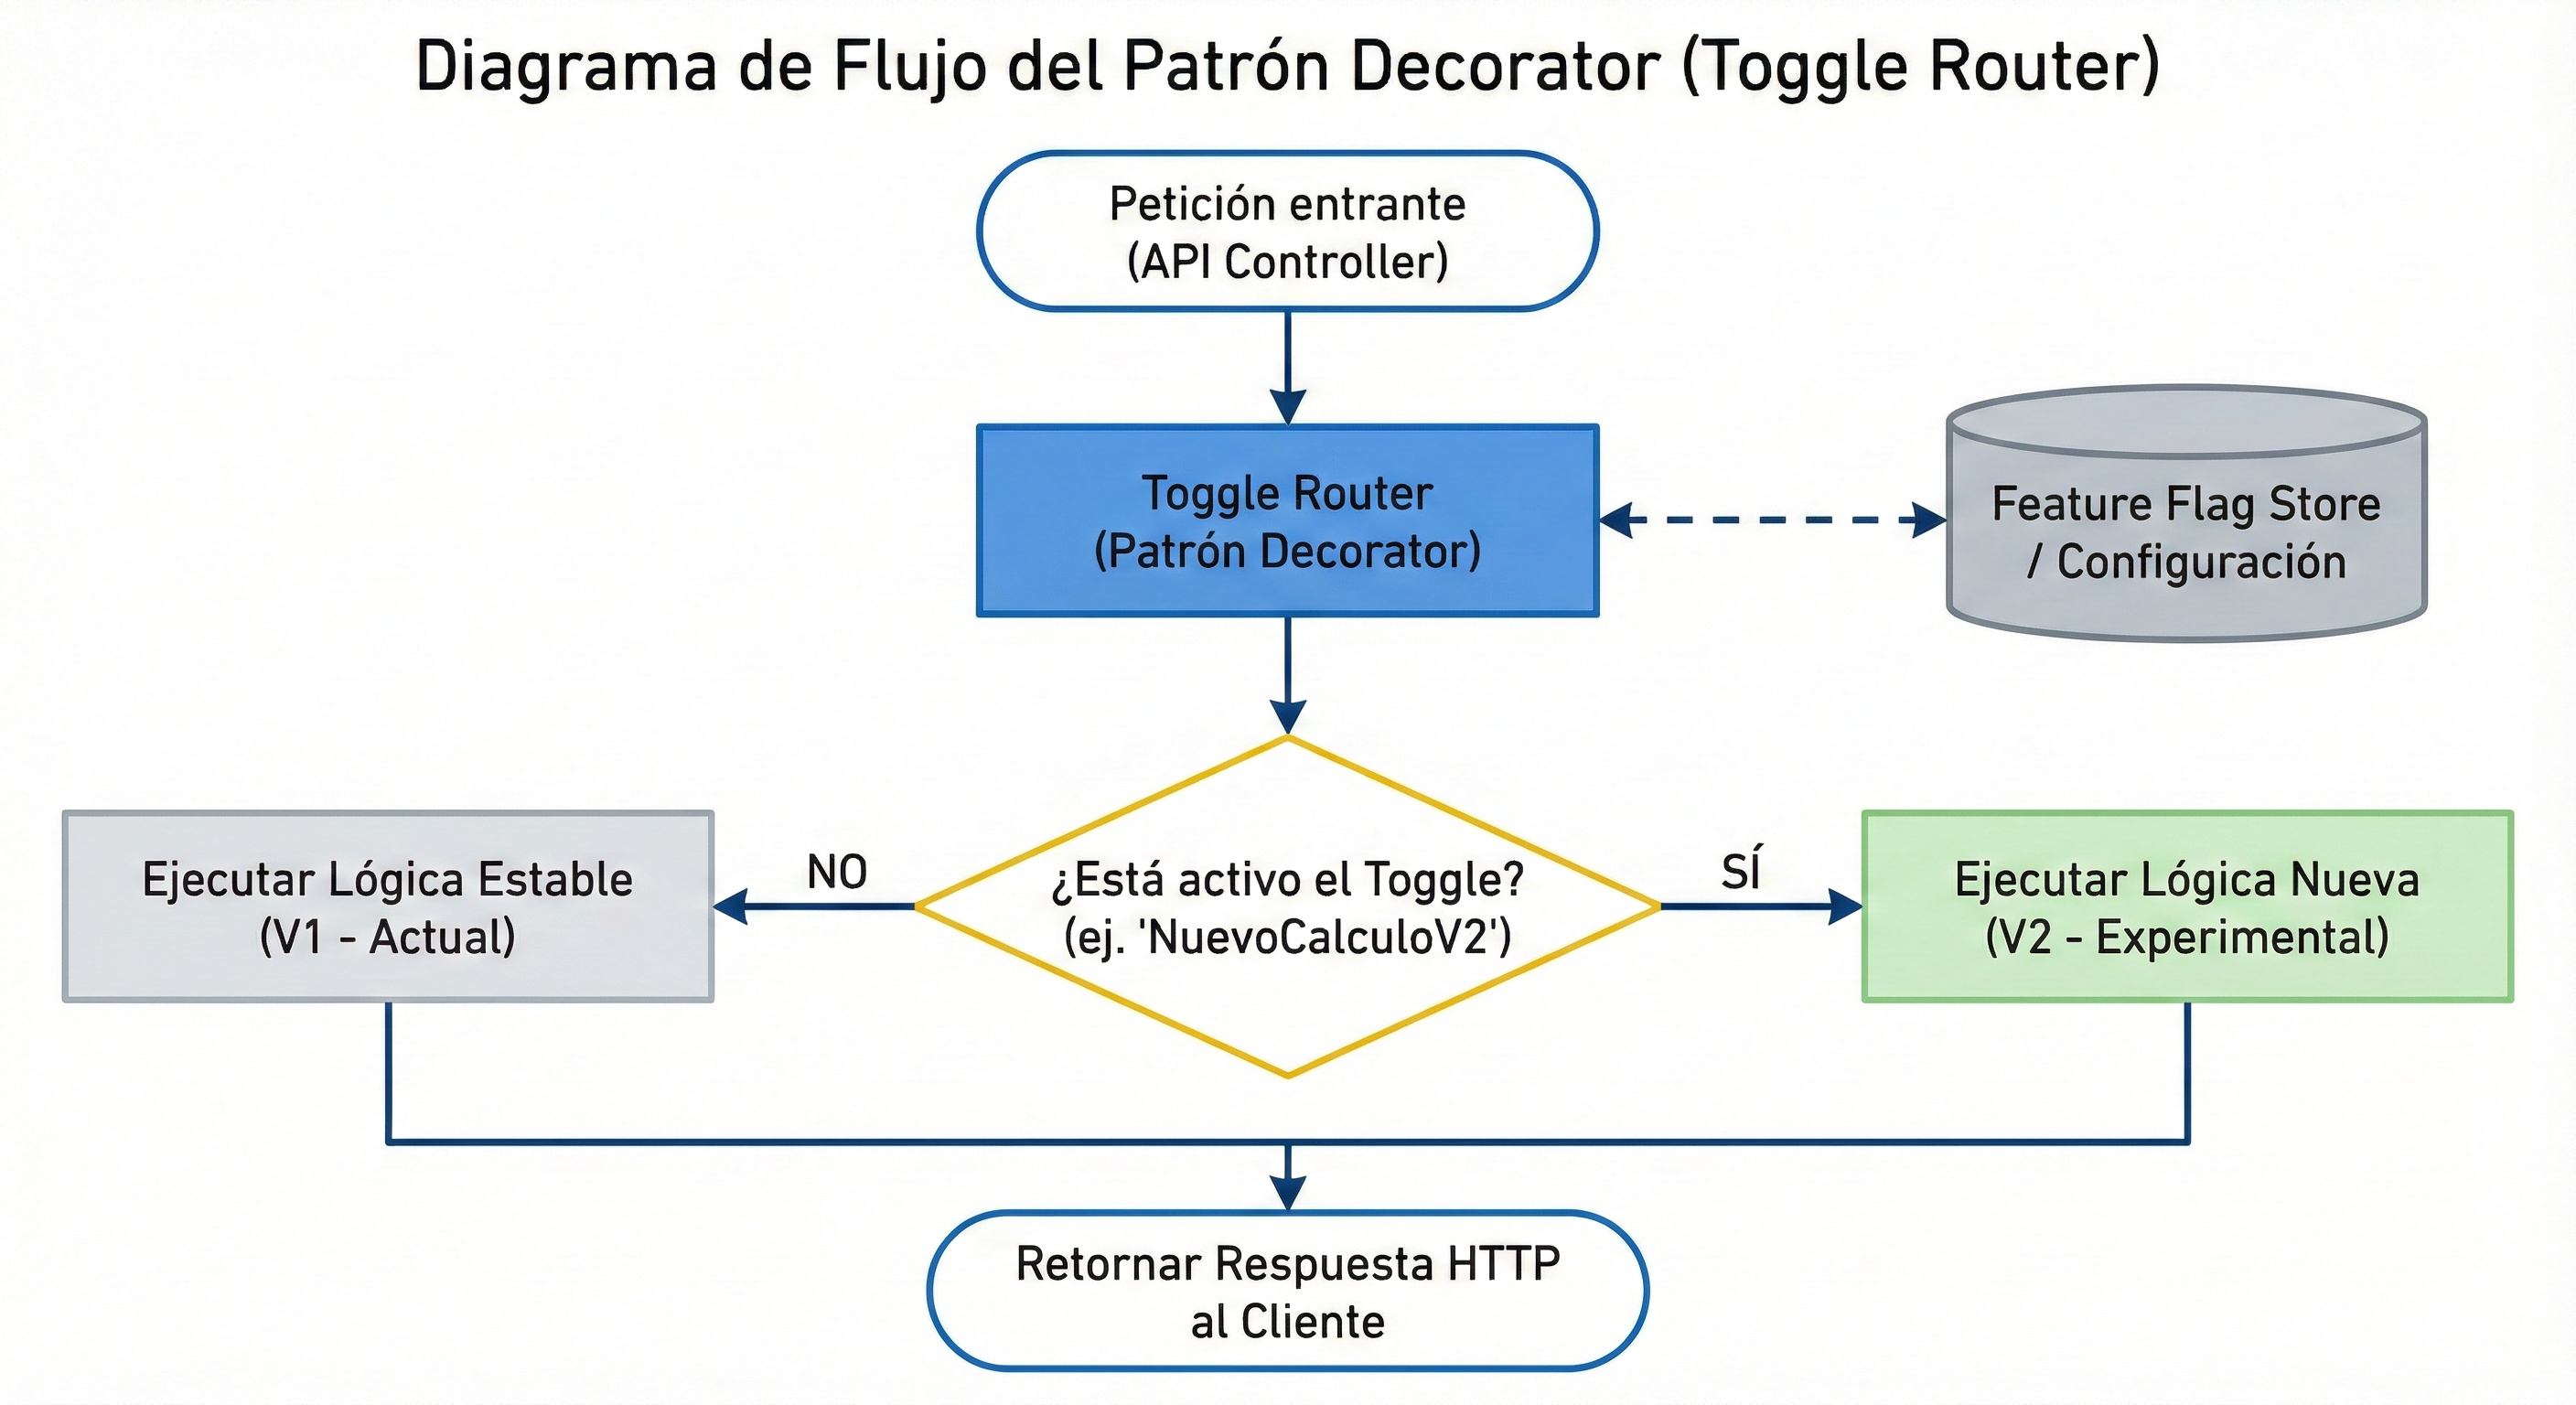
\includegraphics[width=0.95\textwidth]{graphics/flujo_toggle_backend.png}
    \caption{Diagrama de flujo propuesto para el backend. El "Toggle Router" intercepta la petici\u00f3n y decide din\u00e1micamente qu\u00e9 versi\u00f3n de la l\u00f3gica ejecutar bas\u00e1ndose en la configuraci\u00f3n externa, desacoplando el despliegue de la activaci\u00f3n.}
    \label{fig:flujo_backend}
\end{figure*}
% --- FIN DEL BLOQUE DE IMAGEN ---


\subsubsection{Estrategia para el Frontend (Angular)}

En el navegador, el desafío cambia: hay que cuidar los megas del usuario. Por eso, nuestra propuesta descarta el viejo truco de ``ocultar el botón'' y apuesta por una carga perezosa real (\textit{Conditional Lazy Loading}).

La lógica es esta: al entrar, la app solo descarga una lista liviana de ``qué está prendido y qué no''. Si el toggle del ``Mapa Interactivo V2'' está apagado, la librería pesada de mapas ni siquiera viaja a través de la red. Así evitamos saturar el ancho de banda y hacemos que la página vuele, incluso en los teléfonos más modestos.

\subsubsection{Segmentación y Control de Dependencias}

Finalmente, queremos que la activación no sea ``todo o nada''. Adaptando a \cite{chen2025horizon}, diseñamos los toggles para lanzamientos graduales: un productor ``Beta Tester'' podría ver métricas avanzadas mientras el resto sigue con la vista básica.

Y para evitar romper la interfaz, incorporamos reglas de juego. Teniendo en cuenta las advertencias de \cite{hal2022interaction} sobre el caos de las interacciones, el sistema validará jerarquías: no permitiremos activar un toggle hijo (ej. ``Filtros por Vereda'') si su padre (``Búsqueda Avanzada'') está apagado. Es una forma de garantizar integridad por diseño.
